\chapter{The software factory as a distributed system}
\label{ch07-software-factory-distributed-system}
\begin{quote}
\textbf{Evidence profile.} 0 strong \(\cdot\) 4 directional \(\cdot\) 2 corroborating \(\cdot\) 0 null or conflicting evidence items. Four additional sources establish historical lineage but do not provide evidence about agent-system outcomes. This chapter supplies the system model that the practices in Chapters 8 through 19 attach to; it develops no practice of its own.

\textbf{Chapter claim.} The factory, not the worker, owns the reliability promise.
\end{quote}

In one local fault demonstration, described with its limitations in Chapter 9, the worker was killed after an external mutation had been requested and before completion became durable. The naive recovery path sent the request again and reported success. The guarded path issued one request, retained the unresolved state, and stopped for reconciliation. That trial does not estimate a general failure rate. It identifies the boundary this chapter develops: the factory must preserve logical work and effect identity across the failure of the process executing them.

Now consider the same fault without the guard, as a constructed sequence. A worker finishes its task, opens the pull request, and dies before its completion record reaches durable storage. The scheduler sees an unfinished attempt and, correctly by its own lights, schedules another. The second attempt produces a second branch and a second pull request for the same change. The operator's summary reads ``the agent duplicated its work.'' Both attempts may have produced valid work; the duplicate effect arose at the coordination boundary, in the interval between an external effect and the internal record of it, an interval no model improvement can close. The same shape recurs with different surface reports: the model produced a plausible patch, but the process hosting it was evicted before recording completion; the model finished, but a second worker on the same task had already pushed a conflicting branch; the tests passed, but against a repository revision three merges old. These are failures of coordination, durability, versioning, and effect management, and they belong to the machinery around the coding agent's trajectory, not to that trajectory itself.

\hypertarget{when-this-framing-becomes-necessary}{%
\section{When this framing becomes necessary}\label{when-this-framing-becomes-necessary}}

A single coding-agent trajectory, the sequence of model calls, tool calls, and edits one agent performs, is one execution component. It starts, reads state, produces an artifact, and stops. Everything that makes that trajectory count as work belongs to machinery the trajectory does not contain: the scheduler that assigned it, the store that remembers what it was asked to do, the repository state it read and will write, the verifier that decides whether its output is acceptable, the publisher that turns an accepted artifact into an external effect, the external services that accept or reject that effect, and the resource policy that decided this work deserved compute at all. The whole arrangement can be thought of as a \textbf{software factory}: the durable system that accepts logical work, schedules attempts, runs workers, verifies artifacts, publishes effects, and reconciles disagreement between its records and the world. The agent is one worker inside it.

Treating that machinery as an engineered system is not a new idea. Osterweil (\href{https://dl.acm.org/doi/10.5555/41765.41766}{1987}, \href{https://dl.acm.org/doi/10.1145/253228.253440}{1997}) argued that software processes are software too, and Choi and Scacchi (\href{https://www.ics.uci.edu/~wscacchi/Software-Process/Readings/DistSysFactory.pdf}{1991}) described the software factory itself as distributed infrastructure, with the coordination substrate treated as a first-class engineering object; the CNCF's Secure Software Factory reference architecture (\href{https://tag-security.cncf.io/community/working-groups/supply-chain-security/secure-software-factory/secure-software-factory/}{CNCF TAG Security}) supplies the contemporary vocabulary, scoped to supply-chain security rather than fault tolerance. The Sources and evidence section places each of these. Autonomous workers change the failure model. The processes Osterweil programmed and the infrastructure Choi and Scacchi described coordinated deterministic tools and human developers who could be asked what they meant. The modern factory schedules autonomous, nondeterministic workers that edit persistent code, call external APIs, run concurrently with one another, and can claim completion incorrectly. A compiler does not assert that it succeeded when it failed. An agent can, fluently and in detail. Practitioner systems have converged on the same decomposition: OpenAI's Symphony orchestration (\href{https://openai.com/index/open-source-codex-orchestration-symphony/}{OpenAI 2026}) and Cloudflare's issue-triage factory (\href{https://blog.cloudflare.com/astro-issue-triage/}{Cloudflare 2026}) both separate a durable work ledger, a scheduler, disposable workers, and gated publication. These are practitioner cases from the operating teams, corroborating convergence on the decomposition, not controlled evidence that the decomposition improves any measured outcome.

Not every agent deployment needs this frame. A local assistant that reads a repository, proposes a patch in an interactive session, and exits has one process, one human, and no durable coordination state. If the process dies, the human restarts it and loses only convenience. Modeling that as a distributed system would likely add more cognitive overhead than worthwhile.

The frame becomes applicable when any of the following hold:

\begin{itemize}
\tightlist
\item
  useful work must outlive a process, so progress needs a durable record independent of any worker;
\item
  coordination spans components that fail independently, so no single crash can be assumed to take the whole system down cleanly;
\item
  multiple workers act concurrently on versioned or shared state, so ordering and ownership become contested;
\item
  external systems can commit effects asynchronously, so the factory's records and the world can disagree; or
\item
  verification and publication occur in separate failure domains, so an artifact can be verified and never published, or published and never verified.
\end{itemize}

Once any of these conditions holds, the factory need not \emph{be} a distributed system in some essential sense. It exhibits distributed-systems failure modes: lost updates, stale authority, duplicate effects, split-brain records, partial failure. Those failure modes have known engineering treatments, and model capability is then only one contributor to reliability among several.

\hypertarget{the-distinctions-recovery-depends-on}{%
\section{The distinctions recovery depends on}\label{the-distinctions-recovery-depends-on}}

Most factory failures reduce to a conflation of two things the system treated as one, and show up in five distinct categories.

\textbf{Logical work versus execution attempt.} The user's intent, e.g., ``fix this bug once,'' is logical work. A worker process trying to satisfy it is an attempt. One work item may consume many attempts; a retry is a new attempt at the same logical work, not new work. A system that identifies work with its current attempt loses the work when the attempt dies.

\textbf{Lease and liveness versus authority.} A lease, claim, or heartbeat answers an allocation question: who should be working on this now, and is that worker probably alive? It does not answer the safety question: whose writes may be accepted? A worker whose lease expired during a network partition can still be running and still be writing. The mutation boundary must be able to reject it; the lease alone cannot.

\textbf{Candidate artifact versus accepted completion.} A worker producing a branch, a diff, or a message saying the task is done has produced a candidate. Acceptance is a separate event that only independent evidence should trigger. An agent's completion claim is input to verification, never a substitute for it.

\textbf{Local completion record versus external commitment.} The factory recording ``pull request opened'' and the code host having opened the pull request are two facts in two failure domains. Either can exist without the other, as the constructed duplicate-pull-request sequence in the opening shows. A crash between the external effect and the internal record leaves the effect real and the record absent; a crash in the other order leaves the record present and the effect absent. Both cases are normal, and recovery must handle both.

\textbf{Verifier output versus semantic truth.} A green verifier establishes that a specific check, in a specific configuration, against a specific artifact version, did not fail. It does not establish that the change is correct, and a red verifier does not establish that the change is wrong; the verifier itself can time out, flake, or test the wrong revision. Ge and Zhang (\href{https://arxiv.org/abs/2602.02307}{2026}) measured this directly in 1,960 open-source Java projects: 3.2 percent of GitHub Actions builds were rerun, and 67.73 percent of those rerun builds were flaky, affecting 1,055 projects. That is a measurement of rerun builds specifically, not a claim that two-thirds of all builds are flaky, but it is enough to establish that verifier output and software state are distinct signals.

\hypertarget{a-reference-lifecycle-for-logical-work}{%
\section{A reference lifecycle for logical work}\label{a-reference-lifecycle-for-logical-work}}

The distinctions become operational as identities. Each names one fact the factory must be able to recover without asking the failed worker:

\begin{longtable}[]{@{}
  >{\raggedright\arraybackslash}p{(\columnwidth - 2\tabcolsep) * \real{0.3000}}
  >{\raggedright\arraybackslash}p{(\columnwidth - 2\tabcolsep) * \real{0.7000}}@{}}
\caption{Identity vocabulary used through the rest of the book.}\tabularnewline
\toprule\noalign{}
\begin{minipage}[b]{\linewidth}\raggedright
Identity
\end{minipage} & \begin{minipage}[b]{\linewidth}\raggedright
Names
\end{minipage} \\
\midrule\noalign{}
\endfirsthead
\caption[]{Identity vocabulary used through the rest of the book. \emph{(continued)}}\tabularnewline
\toprule\noalign{}
\begin{minipage}[b]{\linewidth}\raggedright
Identity
\end{minipage} & \begin{minipage}[b]{\linewidth}\raggedright
Names
\end{minipage} \\
\midrule\noalign{}
\endhead
\bottomrule\noalign{}
\endlastfoot
\texttt{work\_id} & stable logical work; the intent that should happen once logically \\
\texttt{input\_state\_id} & the repository or repositories, branches, and revisions against which the attempt was planned and executed \\
\texttt{ownership\_epoch} & monotonic generation of write authority over that work \\
\texttt{attempt\_id} & one execution attempt under a given work and epoch \\
\texttt{artifact\_version} & concrete code or state produced by an attempt \\
\texttt{verification\_id} & one verification execution, including the artifact, verifier version, environment, and inputs it observed \\
\texttt{effect\_id} & one logical externally visible mutation; an idempotency key may represent this identity at a boundary \\
\end{longtable}

\texttt{input\_state\_id} is the identity most specific to code work. Without it, the failure ``tests passed against a repository revision three merges old'' can be described but not expressed: nothing in the record says which state the attempt actually observed. For cross-repository work it can point to a manifest of several repository-and-revision pairs. An \texttt{effect\_id} is not itself the destination's idempotency key; the key is one implementation of the identity contract at a boundary that supports it.

Figure \ref{fig:ch07-decomposition} shows how the identities relate. It is a model of identities and boundaries, not a required service architecture. Three obligations follow from it, stated here in their architecture-neutral form. First, no authoritative fact required for recovery or publication should exist only in a worker. A worker may create durable checkpoints, commits, logs, or private attempt references; it cannot unilaterally make them authoritative, and recovery must not depend on the failed worker's private memory. Second, every externally visible effect crosses a named, protected boundary. Third, whenever local and external state can diverge, an owned reconciliation path must exist, because any factory whose publication boundary can crash mid-effect will accumulate record-world disagreements at some background rate.

\begin{figure}[htbp]
\centering
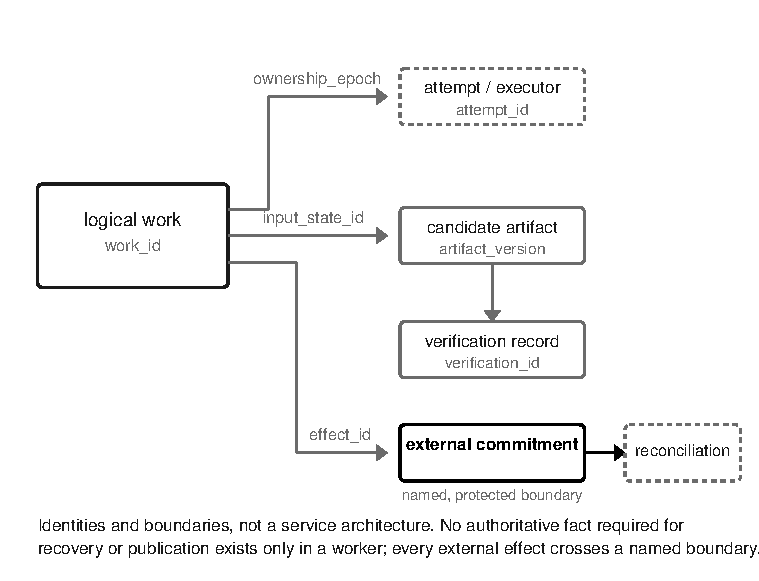
\includegraphics[width=1\textwidth,height=\textheight,keepaspectratio]{figures/ch07-factory-decomposition.pdf}
\caption{The identity and boundary model. Logical work carries an ownership epoch granting authority to an attempt, an input state the attempt observes, and an effect identity for each external commitment. The attempt produces a candidate artifact bound to a verification record; the external commitment is paired with an owned reconciliation path. Authoritative facts live on the work side of each boundary, never only in the worker.}
\label{fig:ch07-decomposition}
\end{figure}

Logical work and attempts move through separate lifecycles, shown in Figure \ref{fig:ch07-state-machine}. The distinction the figure enforces is the one the opening case turned on: the death of an attempt is an event in the attempt lifecycle, and by itself it moves logical work nowhere. Work under an ownership epoch stays owned across a retryable attempt failure; an ordinary retry creates a new \texttt{attempt\_id} under the same epoch, while reassignment to a different executor creates a new epoch. A terminal attempt failure does not terminate the work either; work policy decides whether the work re-enters eligibility, blocks, or fails. Read-only work whose accepted outcome requires no external effect can complete without publication; work whose outcome requires one passes through the effect boundary, and an unresolvable outcome parks the work in \texttt{unknown\_external\_state} or \texttt{reconcile\_required} rather than guessing.

\begin{figure}[htbp]
\centering
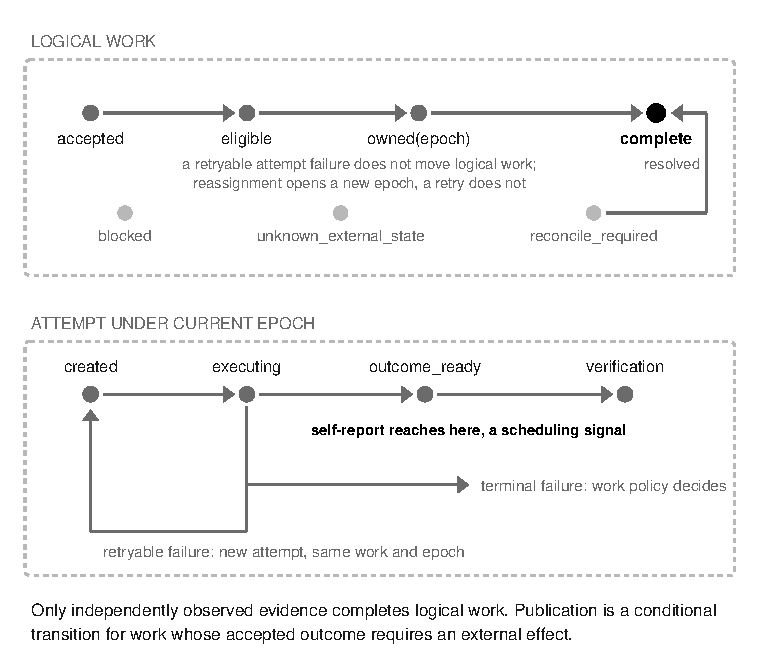
\includegraphics[width=1\textwidth,height=\textheight,keepaspectratio]{figures/ch07-factory-state-machine.pdf}
\caption{Separate lifecycles for logical work and for attempts. Logical work runs accepted, eligible, owned under an epoch, complete, with side states for blocked, unknown external state, and reconciliation. Attempts run created, executing, outcome ready, verification under the current epoch; a retryable failure produces a new attempt under the same work, a terminal failure defers to work policy, and reassignment opens a new epoch. A worker's self-report can move an attempt only to outcome ready; only independently observed evidence completes logical work.}
\label{fig:ch07-state-machine}
\end{figure}

A model saying ``done'' can move an attempt to outcome ready. Only independently observed evidence should complete logical work. The agent's self-report is a scheduling signal, telling the factory an artifact exists and is worth verifying. It is never an acceptance signal.

\hypertarget{six-factory-contracts}{%
\section{Six factory contracts}\label{six-factory-contracts}}

The lifecycle holds only if the factory enforces a set of obligations. Later chapters cite them by identifier (I1 through I11), so the identifiers are stated here; the full normative statements, in machine-testable form, live in the repository artifact \href{https://github.com/sjarmak/engineering-reliable-coding-agents/blob/main/protocols/factory-contracts.yaml}{\texttt{protocols/factory-contracts.yaml}}. They are not all properties of the same kind: some are safety properties, some are liveness or visibility obligations, and some are design rules about recovery code and evidence, so they are grouped here as six contract families rather than presenting them as a uniform formal list.

\textbf{Work continuity and retry identity (I1, I4).} Accepted work cannot silently disappear: every accepted \texttt{work\_id} reaches a terminal state or remains visibly pending. A retry is a new \texttt{attempt\_id} under the same \texttt{work\_id}, never a duplicate work item.

\textbf{Generation-scoped authority (I2, I3).} Only the current \texttt{ownership\_epoch} may commit a mutation at a protected boundary, and a superseded worker must be rejected even if it is still running; this is fencing, enforced at the boundary, not inferred from the lease (I2). A stale completion cannot advance logical state: a durable transition validates generation and attempt identity, not the scheduler's belief about who is running (I3).

\textbf{External-effect safety (I5).} Externally visible effects are safe under redelivery or explicitly uncertain: an idempotency key, an atomic effect-plus-dedup record, natural convergence, adapter-owned reconciliation, or an explicit \texttt{unknown\_external\_state}. No generic exactly-once claim across a boundary that cannot provide it.

\textbf{Record and evidence consistency (I6, I7, I8).} Contradictory durable records trigger reconciliation under declared authority precedence, not guesswork (I6). Evidence is version-bound: a verifier result or retrieved fact is valid only for the \texttt{artifact\_version} or input state it observed (I7). Verifier failure is distinct from software failure: an infrastructure timeout or flake is not a semantic defect, and a pass establishes only what that verifier can detect (I8).

\textbf{Visible liveness and safe recovery (I9, I10).} Admissible work cannot starve invisibly (I9). Recovery preserves the same obligations as normal execution: recovery paths are production code with authority and must be tested as such (I10).

\textbf{Causal attribution (I11).} Consequential transitions are causally attributable: work, attempt, actor, input state, authority generation, requested effect, observed response, and resulting durable state.

None of these contracts mention model quality. A factory can hold all of them while running a non-frontier model, and the result is a system that reliably produces candidates produced as a result of that model quality and accurately reports their status. A factory that violates them while running an excellent model produces potentially excellent candidates it loses, duplicates, or misreports. Model capability does not discharge any of these obligations. A stronger model may change their load and the frequency with which they are exercised, but the factory still owns the controls, durable state, and evidence required to enforce them.

The distributed-systems literature I draw on through Parts III to VI transfers directionally to agent factories unless a claim is restricted to the evaluated system. Chubby's lock generations (\href{https://www.usenix.org/conference/osdi-06/chubby-lock-service-loosely-coupled-distributed-systems}{Burrows 2006}) supply the fencing mechanism behind I2, developed in Chapter 18; Borg and Omega (\href{https://research.google/pubs/large-scale-cluster-management-at-google-with-borg/}{Verma et al. 2015}; \href{https://research.google/pubs/omega-flexible-scalable-schedulers-for-large-compute-clusters/}{Schwarzkopf et al. 2013}) supply admission and shared-state scheduling mechanisms behind I1 and I9, developed in Chapter 19. I transfer their mechanisms, not their constants, and none of this machinery addresses model nondeterminism: durability preserves which stochastic decision occurred, not its correctness.

\hypertarget{audit-one-logical-work-item}{%
\section{Audit one logical work item}\label{audit-one-logical-work-item}}

A model's capabilities can only be evaluated meaningfully in the context of the system in which it operates. The following procedure audits a single work item using only the records the factory already keeps, with no additional infrastructure required.

\begin{enumerate}
\tightlist
\item
  Select one recent work item that produced, or attempted to produce, an external effect.
\item
  Recover its \texttt{work\_id}, \texttt{input\_state\_id}, \texttt{ownership\_epoch}, \texttt{attempt\_id}, \texttt{artifact\_version}, \texttt{verification\_id}, and \texttt{effect\_id}.
\item
  For each of those facts, identify its authoritative owner and the boundary at which any consequential mutation is accepted.
\item
  Determine whether a stale attempt can still modify the ledger, branch, artifact pointer, or external system.
\item
  Determine what the factory records when an external effect may have committed but its acknowledgement is missing.
\item
  Verify that the accepted artifact and its verification record refer to the same immutable version.
\item
  Using the fault harness from Chapter 10, inject either a late completion or a lost acknowledgement and retain the resulting event record.
\item
  Record every question the existing trace cannot answer.
\end{enumerate}

Retain five outputs from the audit: an identity map, an authority map, an effect contract, one fault-injection result, and a list of unobservable assumptions.

The unanswered questions from step 8 are often the audit's most valuable result. Each identifies information the factory would need during a real incident but does not currently record. Chapter 8 begins the engineering work at the containment and authority boundary around a single worker. The chapters that follow develop the ledger, replay, diagnosis, verification, topology, and capacity mechanisms required to make these contracts enforceable and observable.

\section*{Sources and evidence}

\textbf{Historical lineage}

\begin{itemize}
\tightlist
\item
  Osterweil (\href{https://dl.acm.org/doi/10.5555/41765.41766}{1987}), ``Software Processes Are Software Too,'' ICSE, and the retrospective (\href{https://dl.acm.org/doi/10.1145/253228.253440}{1997}). Process-as-program lineage; no evidence about agent systems.
\item
  Choi and Scacchi (\href{https://www.ics.uci.edu/~wscacchi/Software-Process/Readings/DistSysFactory.pdf}{1991}), ``The Software Infrastructure for a Distributed System Factory.'' The factory-as-distributed-infrastructure framing predates this book; the workers it coordinated were deterministic tools and people.
\item
  CNCF TAG Security, \href{https://tag-security.cncf.io/community/working-groups/supply-chain-security/secure-software-factory/secure-software-factory/}{Secure Software Factory reference architecture}. Contemporary factory vocabulary, scoped to supply-chain security rather than fault tolerance; I borrow the vocabulary, not the guarantees.
\end{itemize}

\textbf{Directional evidence}

\begin{itemize}
\tightlist
\item
  Burrows (\href{https://www.usenix.org/conference/osdi-06/chubby-lock-service-loosely-coupled-distributed-systems}{2006}), Chubby, OSDI. The lock-generation sequencer behind fencing (I2); a coordination-service mechanism, not agent evidence, developed in Chapter 18.
\item
  Schwarzkopf et al.~(\href{https://research.google/pubs/omega-flexible-scalable-schedulers-for-large-compute-clusters/}{2013}), Omega, and Verma et al.~(\href{https://research.google/pubs/large-scale-cluster-management-at-google-with-borg/}{2015}), Borg. Shared-state scheduling and admission-control mechanisms behind I1 and I9; their measured parameters do not transfer.
\item
  Ge and Zhang (\href{https://arxiv.org/abs/2602.02307}{2026}), flaky GitHub Actions builds, arXiv:2602.02307. 1,960 Java projects; 3.2 percent of builds rerun; 67.73 percent of rerun builds flaky; 1,055 projects affected. A preprint; cited for the verifier-output-versus-software-state distinction within its rerun-build scope only.
\end{itemize}

\textbf{Corroborating practitioner cases}

\begin{itemize}
\tightlist
\item
  OpenAI (\href{https://openai.com/index/open-source-codex-orchestration-symphony/}{2026}), Symphony orchestration, and Cloudflare (\href{https://blog.cloudflare.com/astro-issue-triage/}{2026}), Astro issue-triage factory. Corroborating convergence on the ledger-scheduler-worker-gate decomposition from the operating teams; not controlled evidence that the decomposition improves any measured outcome.
\end{itemize}
